% Created with jtex v.1.0.20
\documentclass{article}
\PassOptionsToPackage{short, nodayofweek}{datetime}


% Start Curvenote Definitions

% Pass Options Section
% base
\PassOptionsToPackage{normalem}{ulem}
\PassOptionsToPackage{utf8}{inputenc}

% template
\PassOptionsToPackage{framemethod=TikZ}{mdframed}
\PassOptionsToPackage{x11names, svgnames}{xcolor}

%%% PACKAGES

% base
\usepackage{inputenc}
\usepackage{url}
\usepackage{graphicx}
\usepackage{adjustbox}
\usepackage{amssymb}
\usepackage{amsfonts}
\usepackage{amsmath}
\usepackage{enumitem}
\usepackage{nicefrac}
\usepackage{booktabs}
\usepackage{microtype}
\usepackage{hyperref}
\usepackage{ulem}
\usepackage{enumitem}
\usepackage{float}
\usepackage{datetime}
\usepackage{xkeyval}
\usepackage{framed}
\usepackage{doi}

% template
\usepackage{natbib}
\usepackage{fancyvrb}
\usepackage{mdframed}
\usepackage{xcolor}

%%%


%%%% Setup Section

% base
\graphicspath{{.}}
% template
\sloppy
\newenvironment{aside}{\begin{framed}}{\end{framed}}
\newmdenv[linewidth=2pt,linecolor=CornflowerBlue,topline=false,bottomline=false,rightline=false,leftline=true,skipabove=20,skipbelow=20,leftmargin=20,rightmargin=20]{callout}
\newfloat{code}{thp}{loc}
\floatname{code}{Program}
\raggedbottom
\bibliographystyle{abbrvnat}
\setcitestyle{authoryear,open={(},close={)},semicolon,aysep={,}}

% End Curvenote Definitions




% colors for hyperlinks
\hypersetup{colorlinks=true, allcolors=blue}
\hypersetup{
pdftitle={\@title},
pdfsubject={},
pdfauthor={\@author},
pdfkeywords={},
addtopdfcreator={Written in Curvenote}
}

\usepackage{curvenote}

\title{Ch. 7: Forearm EMG with dynamometry}

\newdate{articleDate}{30}{4}{2025}
\date{\displaydate{articleDate}}

\author{\bfseries Erin McKiernan\mdseries\\Universidad Nacional Autónoma de México (UNAM), Open Research Community Accelerator (ORCA)\\\AND\bfseries Saúl A. Saldaña Enciso\mdseries\\\AND\bfseries Angélica Rubio García\mdseries\\}

\begin{document}

\maketitle
\keywords{}

\section{Overview}

In this experimental practical, students learn how to simultaneously record forearm muscle EMG and hand dynamometry. Grip strength is measured by applying forces close to values of 50 N, 100 N, and 200 N at 20s intervals. In addition, maximum voluntary strength tests are performed at longer intervals to verify how long volunteers can sustain this level of effort. Overall, this practical is designed to help students understand the relationship between muscle electrical activity and force produced. The duration of the practical can be as short as 30 minutes or up to 1 hour, depending on the number of arm muscles recorded and the complexity of the different muscle activities explored. While not necessary, it is recommended that students carry out the experimental practical in \href{https://curvenote.com/oxa:EPpXta8zJdzN048lz8AR/hZTnTYzQR5EQmCKX51Wj}{Ch. 1: Muscle physiology and EMG basics }prior to this practical.

\section{Learning objectives}

\textbf{Before} this practical, students should be able to:

\begin{itemize}
\item understand how muscles contract and relax (see \href{https://curvenote.com/oxa:EPpXta8zJdzN048lz8AR/hZTnTYzQR5EQmCKX51Wj}{Ch. 1}), or generate force (see \href{https://curvenote.com/oxa:EPpXta8zJdzN048lz8AR/oZzZ9YkLDYhuIWC3d5Sk}{Ch. 4})
\item explain the types of movement, like extension, flexion, abduction, adduction, etc.
\item describe the technique of EMG recording and how it is used to monitor muscle activity
\end{itemize}

\textbf{During} this practical, students will:

\begin{itemize}
\item investigate the different muscles of the forearm that participate in hand grip and grip strength
\item learn about the technique of dynamometry and its use in obtaining force measurements
\item compare changes in force generation during repeated and sustained muscle contractions
\end{itemize}

\textbf{After} this practical, students should be able to:

\begin{itemize}
\item describe changes in the EMG signal associated with changes in force
\item describe the correlations observed between EMG and dynamometry measurements
\item design additional experiments to explore force generation in other muscles
\end{itemize}

\section{Equipment and materials}

\textbf{For dynamometry:}

\begin{itemize}
\item \href{https://www.vernier.com/product/hand-dynamometer/}{Hand dynamometer} (Vernier, order code HD-BTA)
\item \href{https://www.vernier.com/product/labquest-2/}{LabQuest 2} standalone interface (Vernier)
\item Computer with \href{https://www.vernier.com/product/logger-pro-3/}{Logger Pro software} (Vernier) installed to later view and analyze data (optional), or
\item Computer with Python installed to view and analyze data (optional)
\item Other indications: Remove rings or other jewelry that might interfere with hand grip
\end{itemize}

\textbf{For electromyography:}

\begin{itemize}
\item \href{https://backyardbrains.com/products/muscle-spikerbox}{Muscle SpikerBox} (Backyard Brains)
\item 9V battery to power SpikerBox
\item Round surface electrodes (any medical supply provider)
\item Cables with alligator clips to connect electrodes to SpikerBox (Backyard Brains)
\item Cable to connect SpikerBox to a computer, tablet, or smartphone (Backyard Brains)
\item Computer, tablet, or phone with free Backyard Brains \href{https://backyardbrains.com/products/byb-spike-recorder}{Spike Recorder software} installed
\item Phone or tablet adaptor, 3.5mm aux to USB-C (if no aux port on devices; any provider)
\item Alcohol and cotton swabs to help remove electrodes after recording (optional)
\item Other indications: Wear loose sleeves or no sleeves to permit electrode placement
\end{itemize}

\section{Background}

\subsection{Force generation in muscles}

In\href{https://curvenote.com/oxa:EPpXta8zJdzN048lz8AR/hZTnTYzQR5EQmCKX51Wj}{Ch. 1} and\href{https://curvenote.com/oxa:EPpXta8zJdzN048lz8AR/oZzZ9YkLDYhuIWC3d5Sk}{Ch. 4}, we detailed the physiological bases underlying muscle contraction and force generation in muscle, so we will only do a brief overview here. However, this chapter goes into a bit more depth on both the molecular and neural mechanisms.

At the molecular level, force is generated due to the interaction between the cytoskeletal element actin and the molecular motor myosin \citep{rassier2017sarcomere, Rassier2025Mechanisms}. In skeletal muscle, actin and myosin filaments are organized in parallel and with distinct spacing to form a specialized structure called a sarcomere. When actin and myosin bind, the myosin protein heads (the `myosin lever arm') move in what is known as a power stroke, causing the actin filaments to slide toward the sarcomere midline. This action shortens the sarcomere and generates tension. (This is the sliding filament model we saw in \href{https://curvenote.com/oxa:EPpXta8zJdzN048lz8AR/hZTnTYzQR5EQmCKX51Wj}{Ch. 1}.) Thus, as \citet{Rassier2025Mechanisms} write, ``Myosin II is an enzyme that \textbf{converts chemical energy into mechanical work}: a molecular motor that harnesses the free energy released by adenosine triphosphate (ATP) turnover \textbf{to produce force} while interacting with actin filaments'' (emphasis added). We saw previously (\href{https://curvenote.com/oxa:EPpXta8zJdzN048lz8AR/hZTnTYzQR5EQmCKX51Wj}{Ch. 1}) that the amount of force or tension developed in muscle depends on the degree of resting overlap between actin and myosin myofilaments. This is known as the length-tension relationship \citep{}Figure \%s ``.

\begin{figure}[!htbp]
\centering
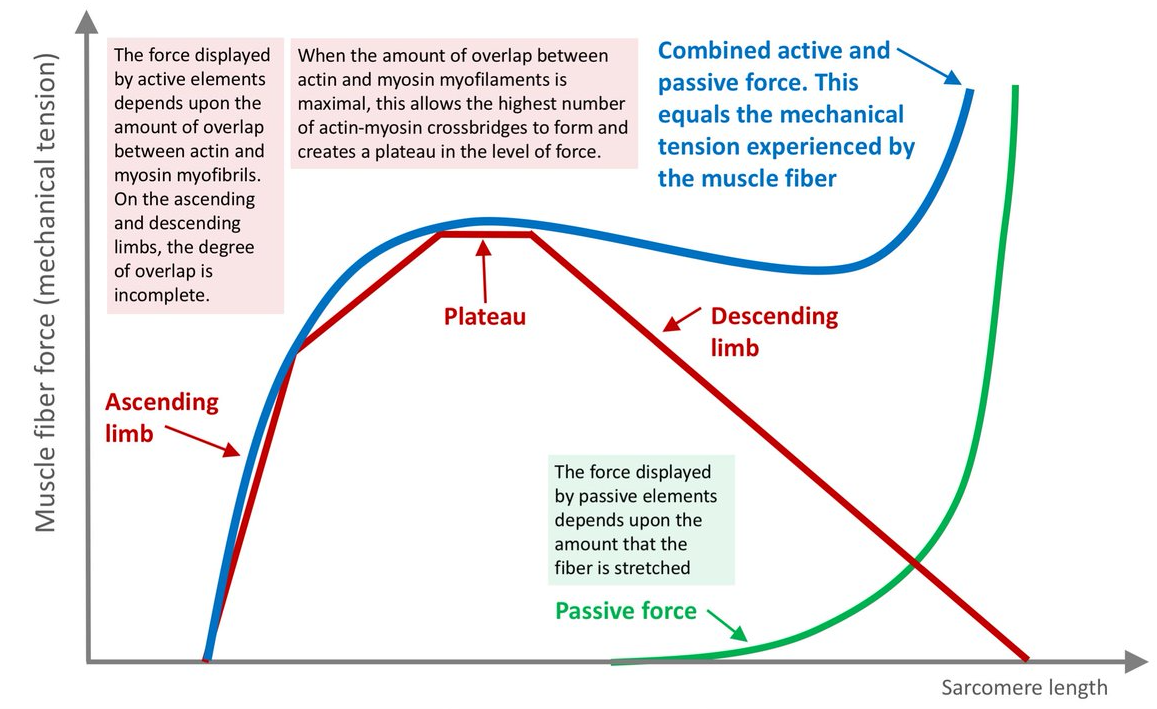
\includegraphics[width=0.9\linewidth]{files/EPpXta8zJdzN048lz8AR-1f4604f22b1712e3532278f27c9f6c4c.png}
\caption[]{Force production in muscle due to active (contraction; red), passive (stretch; green), and combined (blue) forces. The active curve specifically shows the optimal sarcomere length (i.e. degree of myofilament overlap) to generate maximal force during contraction. Image credit: Original source unknown (multiple sources), obtained from Chris Beardsley \href{https://x.com/SandCResearch/status/1116234624412409856}{https://x.com/SandCResearch/status/1116234624412409856}.}
\label{MlwkqfVYNC}
\end{figure}

Moving up organizational levels, as sarcomeres are laid out in series along the length of the muscle fiber, many sarcomeres shortening at once will causes a shortening in the fiber \citep{rassier2017sarcomere}. If this then occurs in the many fibers that make up a larger muscle, the muscle itself will shorten, pulling on tendons and thereby generating force. As \citet{Rassier2025Mechanisms} write, ``In such an arrangement, the molecular effects of myosin-induced sliding of actin give shortening of the muscle with a velocity that is equal to the half-sarcomere shortening, multiplied by the total number of half-sarcomeres along the muscle. It also \textbf{produces a total force that represents the average half-sarcomere force times the number of half-sarcomeres per muscle cross section}'' (emphasis added).

As we saw in\href{https://curvenote.com/oxa:EPpXta8zJdzN048lz8AR/oZzZ9YkLDYhuIWC3d5Sk}{Ch. 4}, when muscles need to generate varying levels of force, there are mechanisms that act at both the neural and muscular levels. Within the muscle, greater force is achieved by recruiting additional motor units (MUs) \citep{openStax_neuro}. Since the activity of all the active MUs in a muscle can sum, more MUs means greater force production. Furthermore, the MUs recruited as more force is needed have different properties, namely that the innervated muscle fibers are typically larger and can individually generate larger forces \citep{Mendell2005size}. (This is the size principle we saw in \href{https://curvenote.com/oxa:EPpXta8zJdzN048lz8AR/oZzZ9YkLDYhuIWC3d5Sk}{Ch. 4}) . Within each MU, the rate at which they fire action potentials (rate coding) is also important for force production \citep{}Figure \%s ``, but is often an ``underappreciated contribution'' \citep{enoka2017rate}. As \citet{enoka2017rate} write, ``The 75\% discrepancy between the sum of the motor unit forces produced by minimal discharge rates and the peak force that can be achieved underscores the significant role of rate coding in the control of muscle force''. Firing rates of MUs are determined largely by neural drive, but also by the intrinsic properties of motor neurons (MNs) such as ionic currents that underlie ``self-sustained firing'' \citep{heckman2004physiology}.

\begin{figure}[!htbp]
\centering
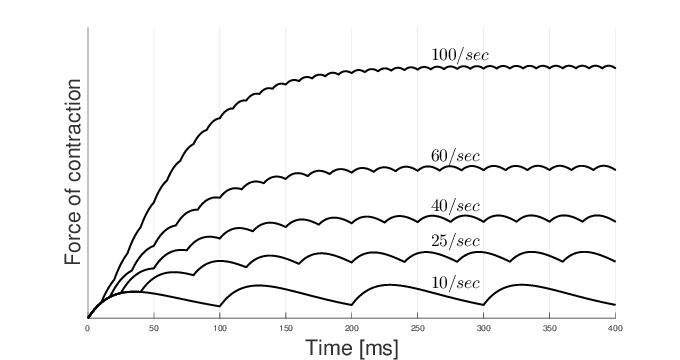
\includegraphics[width=0.8\linewidth]{files/EPpXta8zJdzN048lz8AR-b1e9fbe07b082d58952602b11cad6575.png}
\caption[]{``Force of contraction of a single muscle fiber as a function of time for various motor neuron firing rates. Wave summation effect creates variability allong time.'' Text and image from: Manriquez et al. (2017). Modeling Laryngeal Muscle Activation Noise for Low-Order Physiological Based Speech Synthesis. Interspeech 2017 \cite{Manr_quez_2017}.}
\label{WeuzouGn9A}
\end{figure}

\subsection{Muscles of the forearm}

In the human forearm, there are twenty muscles of varying size and length, and found at different depths \citep{openStax_upper, mitchell2023forearm}. Figure~\ref{b2doQoZWdZ} shows the muscles located on either the anterior (palmar) or posterior (dorsal) side of the forearm, further dividing them into superficial or deep muscles. Note that because we will not be focusing in this practical on displacements of the whole forearm like those involved in extension and flexion at the elbow joint. the biceps brachii, brachialis, and brachioradialis are not covered here (though see \href{https://curvenote.com/oxa:EPpXta8zJdzN048lz8AR/pIDHVE4gOQaQL1y9Os3r}{Ch. 6: Dual EMG recordings of muscle pairs}). Instead, the focus will be on some of the extensors, flexors, abductors, and adductors of the fingers, hands, and wrists. (Additional muscles of the fingers and hands are covered later in \href{https://curvenote.com/oxa:EPpXta8zJdzN048lz8AR/Fwnarvyq1j9AlkJ1JWeF}{Ch. 10: Instrumentation of a simple myoelectric prosthetic}.)

\begin{figure}[!htbp]
\centering
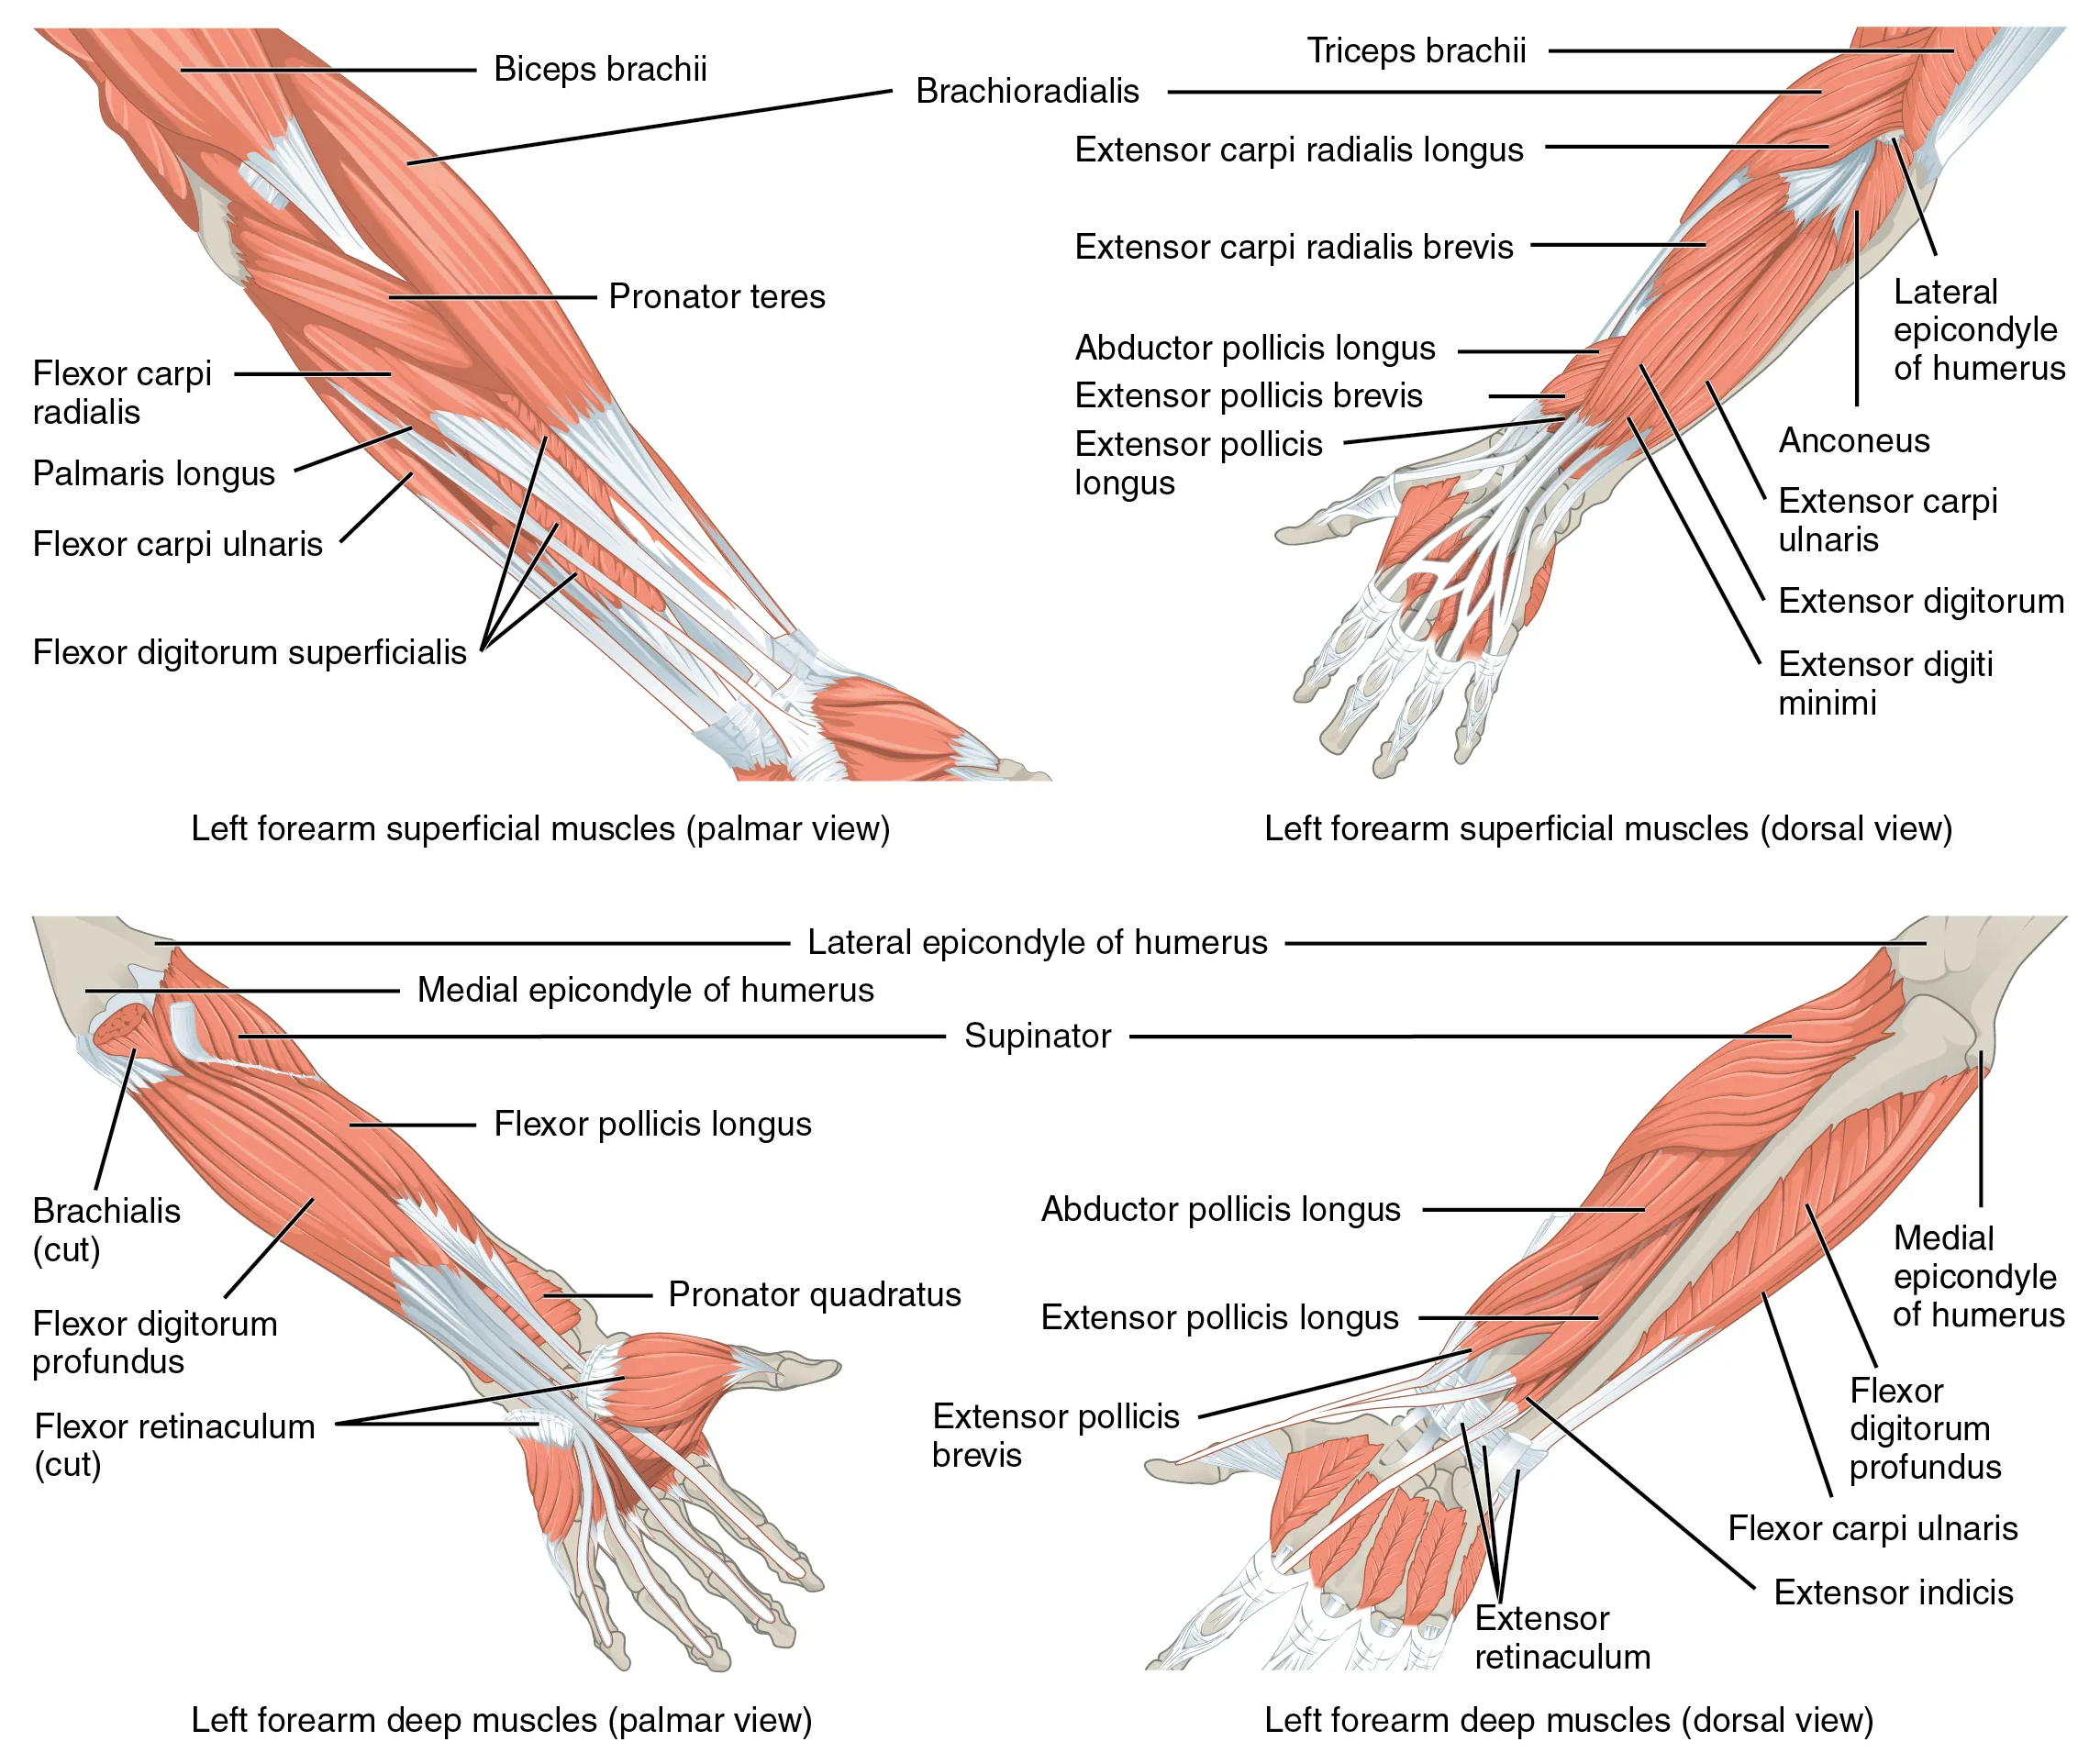
\includegraphics[width=0.9\linewidth]{files/EPpXta8zJdzN048lz8AR-150be6c36065bf3970e44f8e481fd96b.png}
\caption[]{Superficial and deep muscles of the forearm. Image credit: Adapted from OpenStax, CC BY 4.0, via Wikimedia Commons \href{https://upload.wikimedia.org/wikipedia/commons/7/73/1120\_Muscles\_that\_Move\_the\_Forearm.jpg}{https://upload.wikimedia.org/wikipedia/commons/7/73/1120\_Muscles\_that\_Move\_the\_Forearm.jpg}}
\label{b2doQoZWdZ}
\end{figure}

Because the EMG technique here can only record from superficial muscles, we will focus on these, their locations, and different functions. Text in the following sections is pulled from tables in \citet{openStax_upper}.

\subsubsection{Superficial anterior compartment of forearm}

\begin{itemize}
\item \textit{flexor carpi radialis}: bends wrist toward body; tilts hand to side away from body (i.e. flexion and abduction at the wrist and hand, respectively)
\item \textit{flexor carpi ulnaris}: assists in bending hand up toward shoulder; tilts hand to side away from body; stabilizes wrist (i.e. flexion and adduction of the wrist and hand)
\item \textit{flexor digitorum superficialis}: bends fingers to make a fist (i.e. flexion in fingers 2-5)
\item \textit{palmaris longus}: assists in bending hand up toward shoulder (i.e. wrist flexion)
\end{itemize}

\begin{figure}[!htbp]
\centering
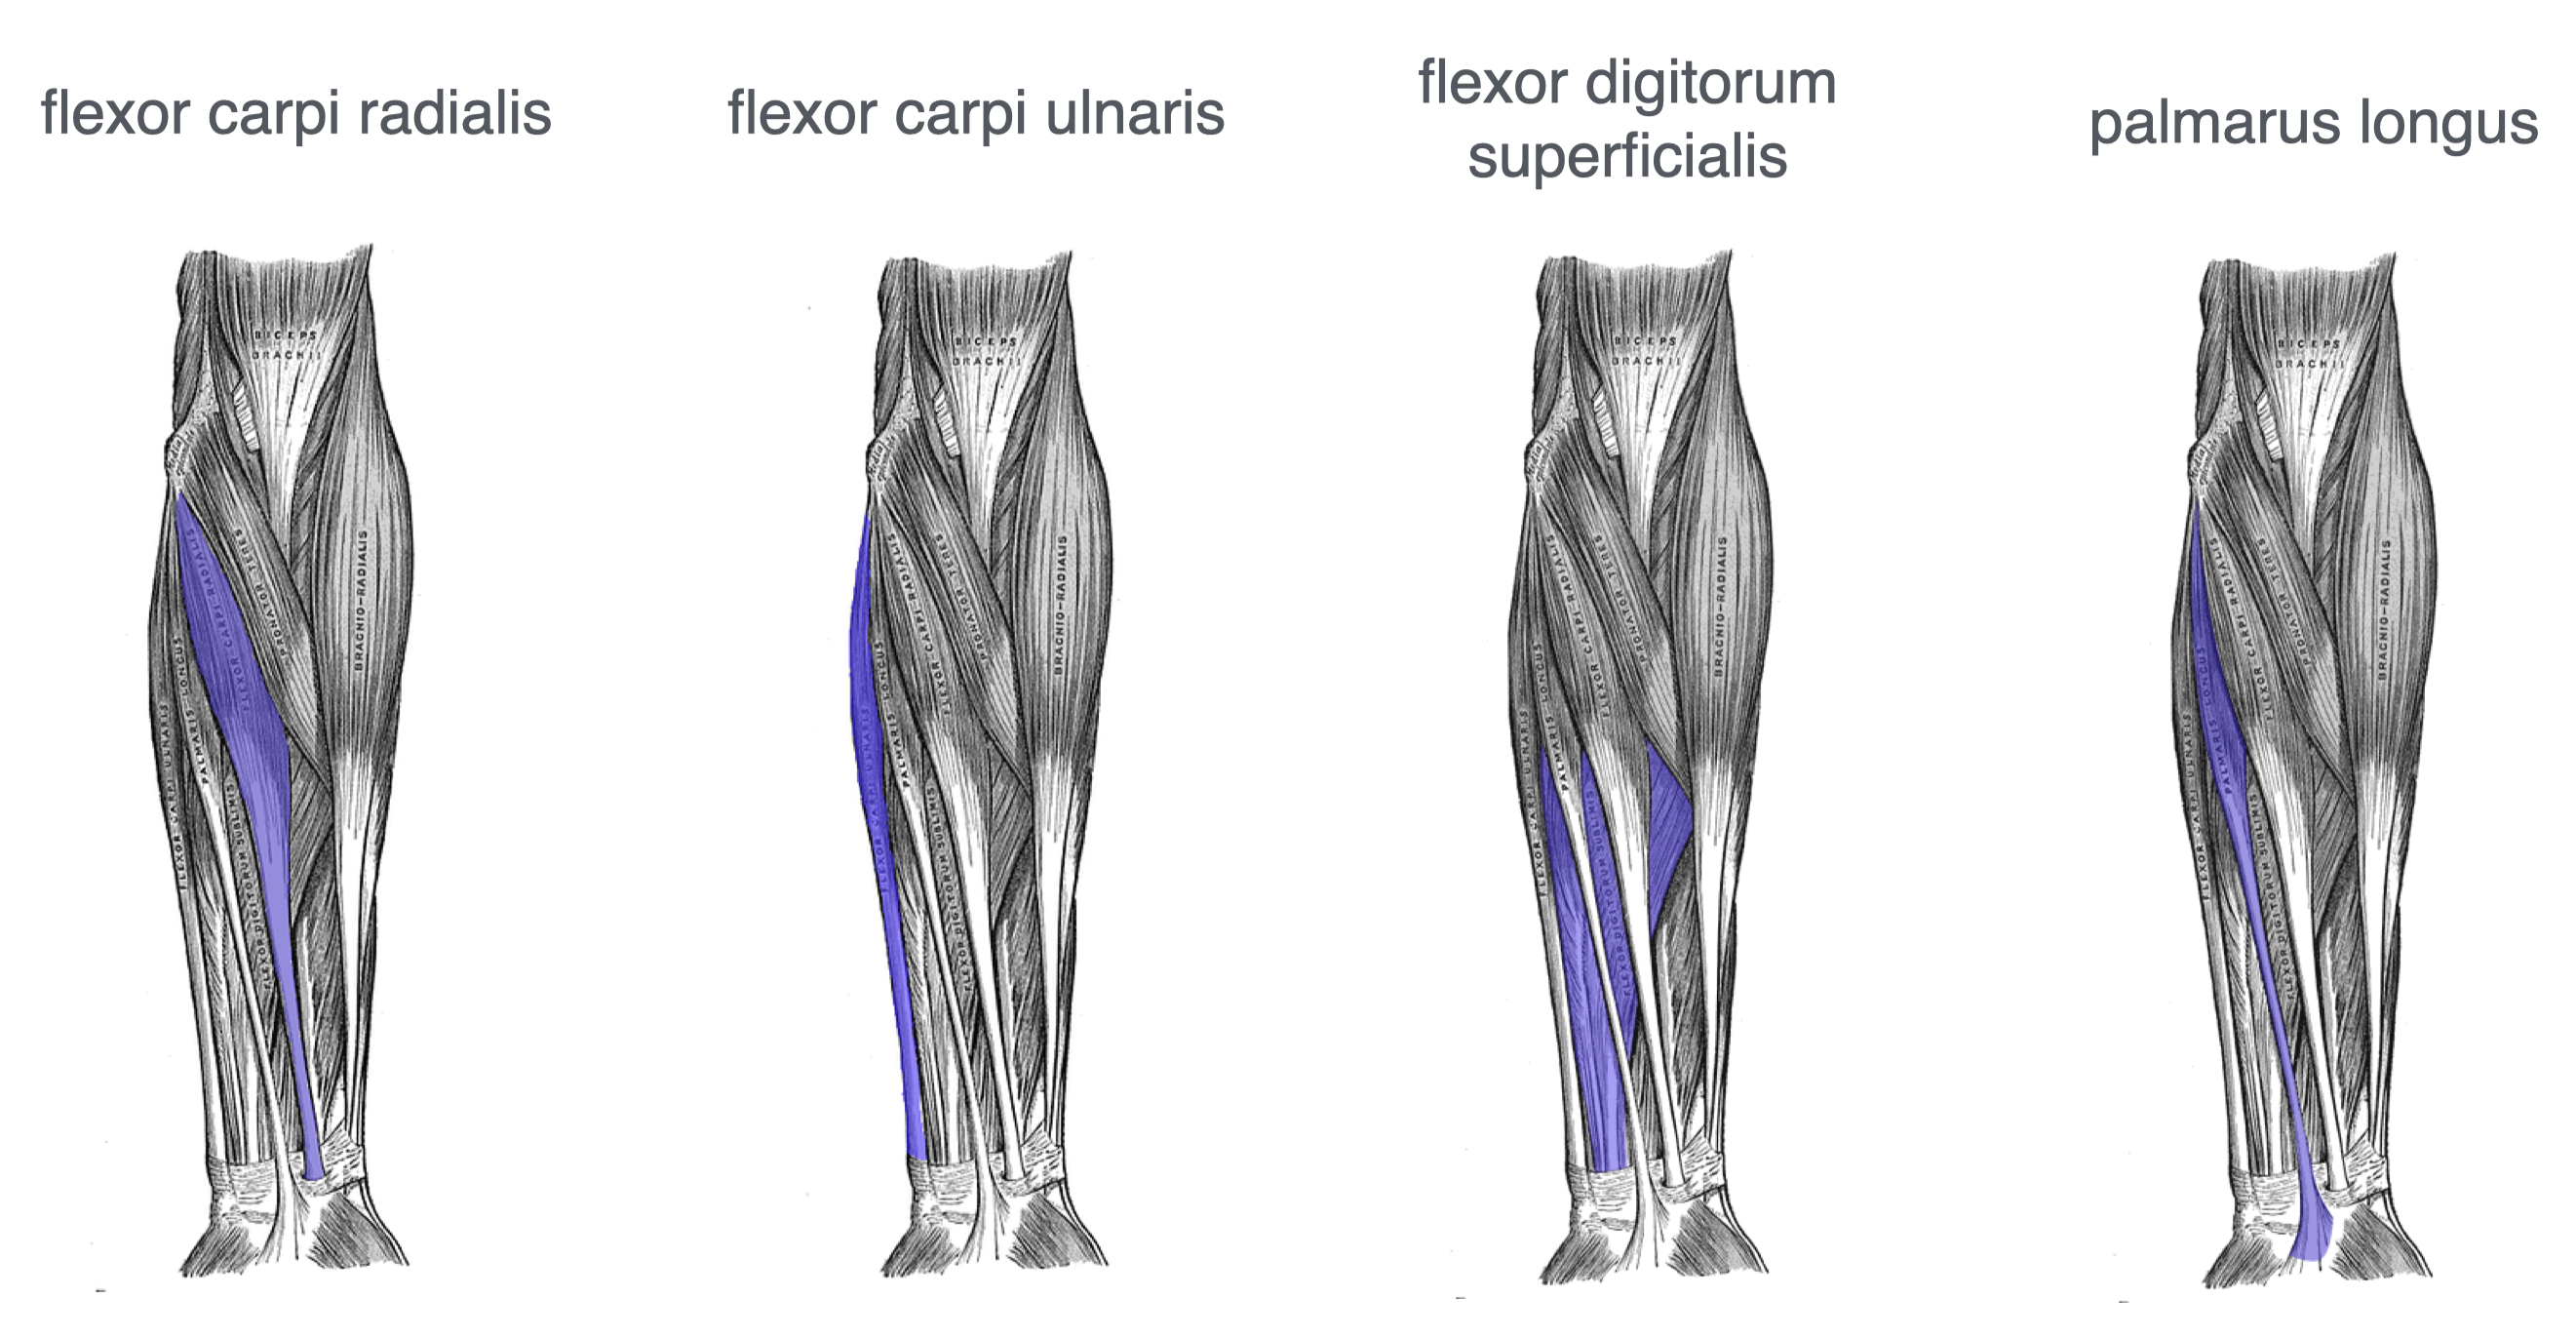
\includegraphics[width=0.9\linewidth]{files/EPpXta8zJdzN048lz8AR-4c33b2f18997f548f79509bf715e4771.png}
\caption[]{Muscles of the superficial anterior compartment of forearm. Each muscle is highlighted in purple to distinguish more easily. Base images from Gray's Anatomy, public domain.}
\label{ZPEeWRuWdh}
\end{figure}

\textbf{Study questions}

\begin{enumerate}
\item Will you be able to record from any of the forearm muscles shown in Figure~\ref{b2doQoZWdZ}? Why, or why not?
\item Will the forearm muscles shown in Figure~\ref{ZPEeWRuWdh} be equally easy to record? To support your answer, take a copy of the figure and draw where you would need to place the EMG electrodes for each muscle.
\item What challenges might you face in recording the forearm muscles, especially if focusing on grip force as measured by the dynamometry?
\end{enumerate}

\subsubsection{Superficial posterior compartment of forearm}

\begin{itemize}
\item \textit{extensor carpi radialis brevis}: assists extensor radialis longus in extending and abducting wrist; also stabilizes hand during finger flexion
\item \textit{extensor carpi radialis longus}: straightens wrist away from body: tilts hand to side toward body (i.e. extension and adduction of the wrist)
\item \textit{extensor carpi ulnaris}: straightens wrist away from body; tilts hand to side toward body (i.e. extension and adduction of the wrist)
\item \textit{extensor digiti minimi}: extends little finger
\item \textit{extensor digitorum}: open fingers and moves them sideways away from body (i.e. extension and abduction of wrist and fingers)
\end{itemize}

\begin{figure}[!htbp]
\centering
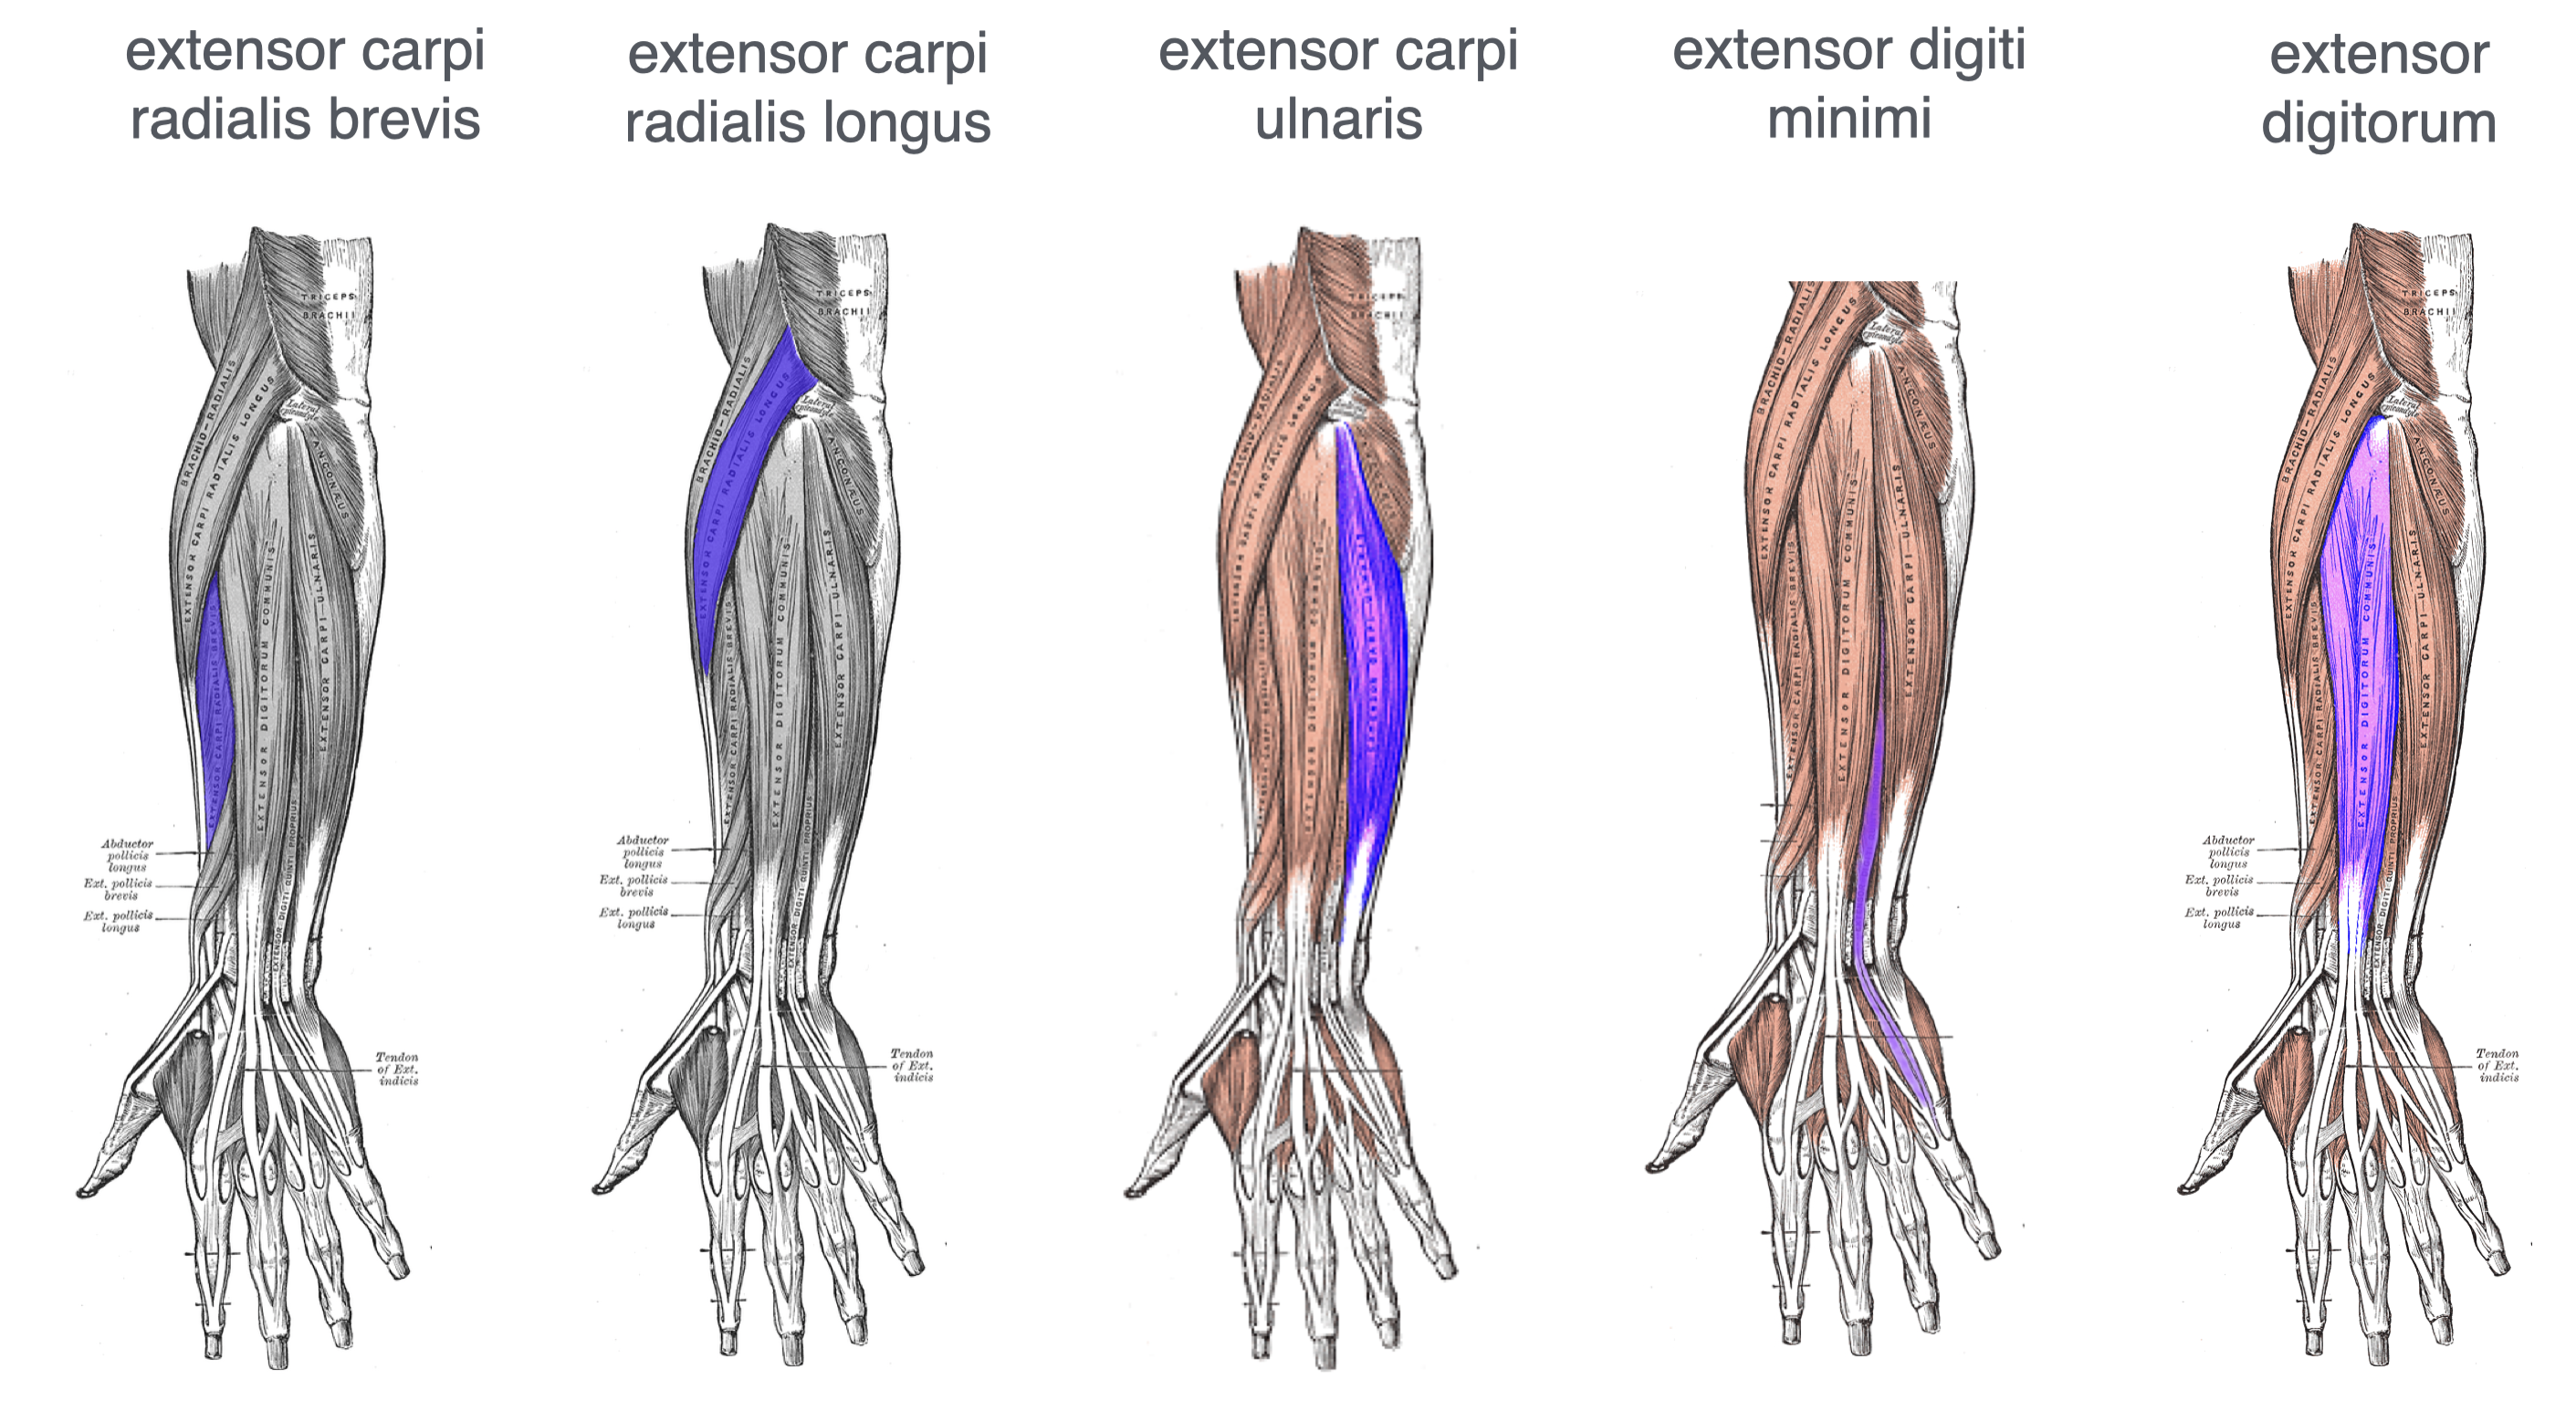
\includegraphics[width=0.9\linewidth]{files/EPpXta8zJdzN048lz8AR-f0bad1de4554c717f552a071f01510df.png}
\caption[]{Muscles of the superficial posterior compartment of forearm. Each muscle is highlighted in purple to distinguish more easily. Base images from Gray's Anatomy, public domain.}
\label{jlCMu7lmVf}
\end{figure}

\textbf{Study questions}

\begin{enumerate}
\item Will the forearm muscles shown in Figure~\ref{jlCMu7lmVf} be equally easy to record? To support your answer, take a copy of the figure and draw where you would need to place the EMG electrodes for each muscle.
\item Given that we will be focusing on grip force as measured by the dynamometry, which of any of the above muscles will be activated during that action?
\item Considering the muscles in Figure~\ref{ZPEeWRuWdh} and Figure~\ref{jlCMu7lmVf}, which do you think will be the best candidates to record from for this experiment? Explain your answer.
\item Are there other places we could record that are not located in the forearm and would be activated?
\end{enumerate}

\subsection{Force and dynamometry}

In physics, force is defined as ``a push or pull on an object with a specific magnitude and direction'' \citep{physicsBook}, or ``that which causes an object to accelerate'' \citep{serway2000physics}. But as the authors of Joint Structure and Function point out, ``Although a force is most simply described as a push or a pull, it is also described as a ``theoretical concept'' because only its effects (acceleration) can be measured'' \citep{levangie2011joint}. This brings us to the well-known equation: $F = ma$. In other words, to calculate the force applied to a given object, we need to know the mass of that object and its acceleration, and take the product of the two. Force is measured in units of kg-m/sec\textsuperscript{2}, or what in the International System of Units (SI) is called a newton (N) \citep{serway2000physics}. Forces can be either external (acting from outside), or internal (produced within the body) \citep{levangie2011joint}. Force generation in muscles is an example of an internal force. Consider the biceps brachii. In concentric contraction, the muscle shortens, thereby producing a force that pulls on the radius bone (via the tendon) and causes bending (flexion) at the elbow joint.

In\href{https://curvenote.com/oxa:EPpXta8zJdzN048lz8AR/oZzZ9YkLDYhuIWC3d5Sk}{Ch. 4}, we discussed how EMG recording can be used to study force generation and fatigue in muscles, showing changes in both amplitude and frequency of the electrophysiological signal when force varies. While this can be a useful measure, it is an indirect one and has limitations. As \citet{levangie2011joint} write, ``\dotsneither electrical activity nor number of motor units is a measure of absolute force generated by a muscle because different motor units produce different tension under different conditions''. Ideally, we would have an independent measure of force that could accompany our EMG recording to correlate the two measures, or detect when discrepancies exist. One reliable way to measure force in muscles is with handheld dynamometry (HHD), which is commonly used in clinical settings to evaluate muscle strength \citep{kolber2005strength, mendoza2014muscle}. HHD presents a number of advantages, including the typically small size and portability of the devices, non-invasiveness of the technique, and ability to measure force directly in newtons. In some cases, a tester must hold the device against the muscle of interest while the subject exerts force. In the special cases of grip or pinch strength, there are dynamometers that the subject can hold themselves and press to measure force \citep{}Figure \%s ``.

\begin{figure}[!htbp]
\centering
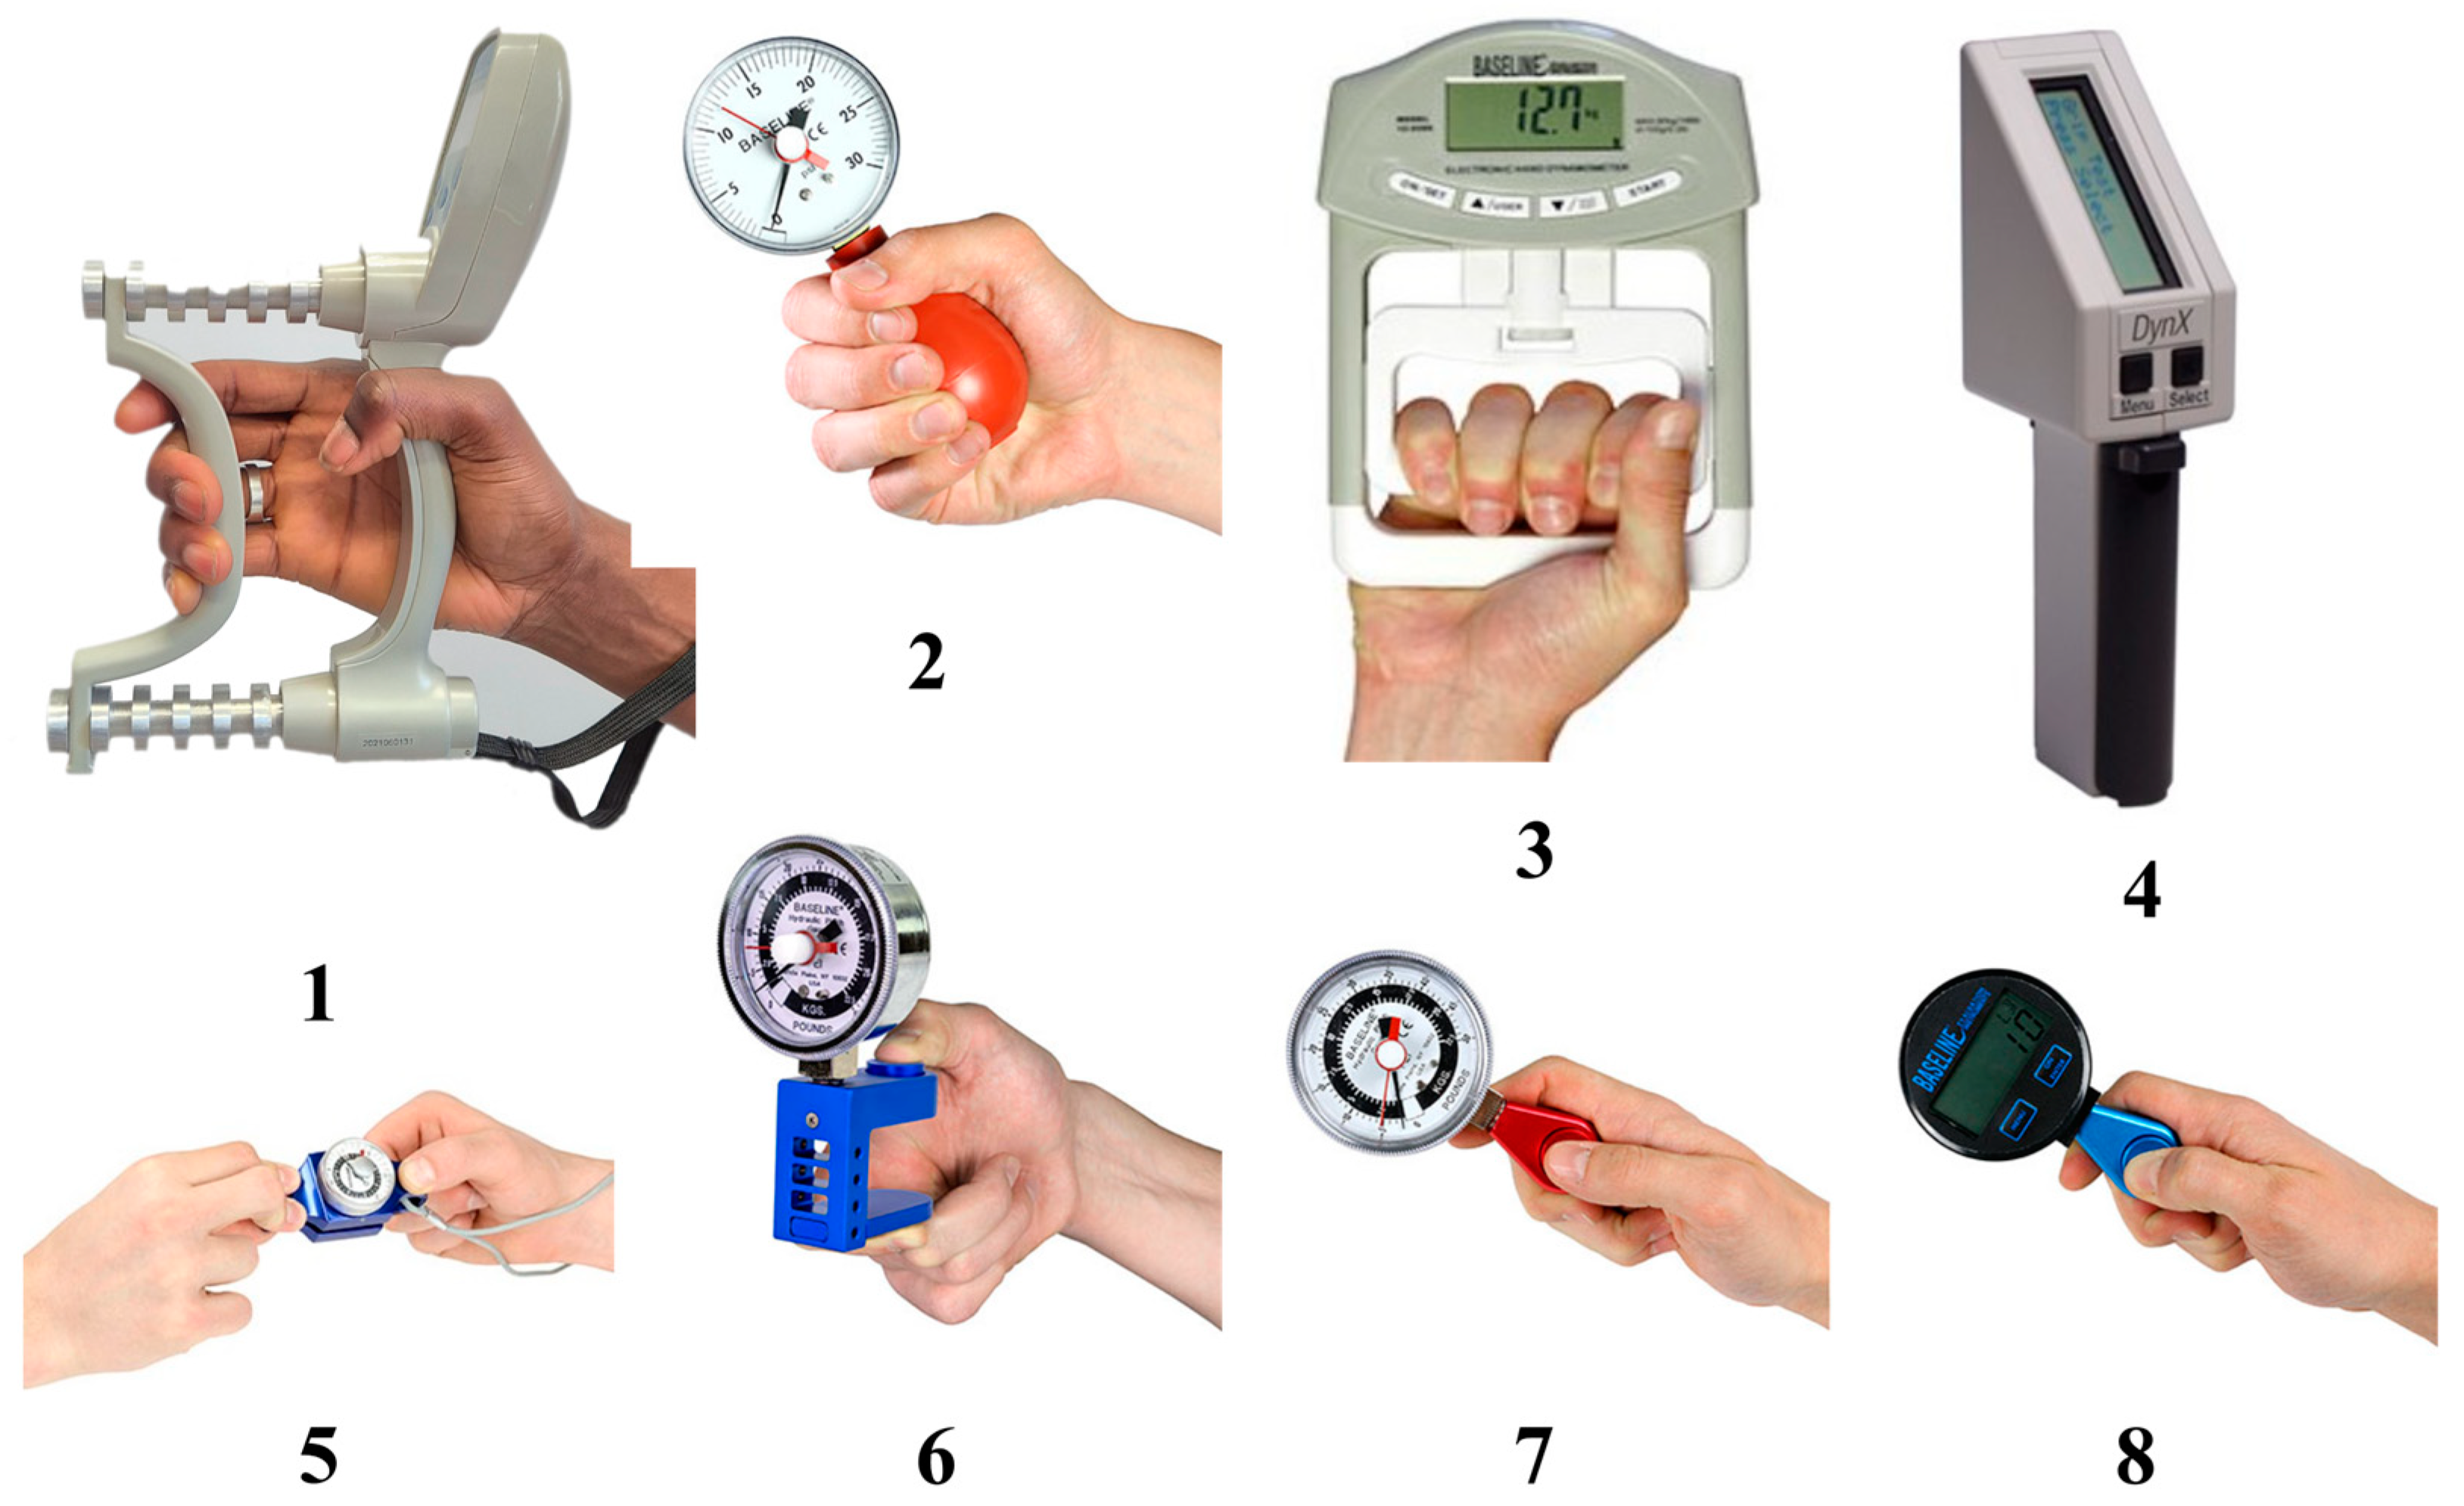
\includegraphics[width=0.9\linewidth]{files/EPpXta8zJdzN048lz8AR-34ccfc6a036ea71458794d37f0a86940.png}
\caption[]{Tools for measuring grip and pinch strengths: (\textbf{1}) Jamar dynamometer; (\textbf{2}) Martin vigorimeter; (\textbf{3}) Smedley dynamometer; (\textbf{4}) Dyn X dynamometer; (\textbf{5}) mechanical pinch gauge; (\textbf{6}) five-position hydraulic pinch gauge; (\textbf{7}) hydraulic pinch gauge; and (\textbf{8}) digital pinch gauge. Image credit: Bergeron \& Kajganic (2024). Sensors, 24(17), 5768; \cite{bergeron2024pressure}}
\label{TosSycwkOy}
\end{figure}

Hand dynamometers vary in terms of the mechanism used to transmit and measure force --- some use a spring, some are hydraulic, some are pneumatic \citep{bergeron2024pressure}. According to \href{https://www.vernier.com/manuals/hd-bta/}{Vernier's specifications}, the dynamometer we will use is a strain-gauge based isometric force sensor, but other models and types could be used to perform the same experiments.

\section{Experimental protocol}

Before carrying out this practical, it is recommended that students perform (or at least read through) the practical described in \href{https://curvenote.com/oxa:EPpXta8zJdzN048lz8AR/hZTnTYzQR5EQmCKX51Wj}{Ch. 1: Muscle physiology and EMG basics }to familiarize themselves with the recording equipment and software. Carry out the steps in stage 1 and 2 of the Ch. 1 experimental protocol to set up the recording device and test the EMG recordings before beginning the force protocols described below. Follow the instructions in \href{http://www2.vernier.com/manuals/labquest2\_user\_manual.pdf}{Vernier's LabQuest\textregistered  2---User Manual} to set up the recording interface, and their product page to set up the \href{https://www.vernier.com/manuals/hd-bta/}{hand dynamometer}.

\subsection{Sustained contractions at one force level}

\begin{enumerate}
\item Place two surface electrodes over the forearm muscle of interest, in parallel with the muscle fibers, and one on the back of the hand or wrist to serve as the reference/ground; [Based on the exercises in Section~\ref{X19Qa0fb3o}, we won't name a specific muscle here (you need to determine which is best); You can also record from different muscles to compare their responses.]
\item Ask the volunteer to rest their arm on the table such that they are completely relaxed and the muscle being recorded is not generating tension
\item Test the EMG recording with the muscle at rest for a few seconds to check there is no activation or noise
\item Set up the LabQuest interface and connect the dynamometer (see links above)
\item Ask the volunteer to hold the dynamometer in their hand in a position that will allow them to press down on the sensor and vary their force; They may need to lift their arm off the table a bit so the sensor and cables can hang down
\item On the next trial, make sure that the dynamometer and the EMG devices are recording; You may need help from a partner to make sure the recordings begin at the same time
\item Once you start your recordings, ask the volunteer to remain at rest for the first 5-10 s, then press on the dyanomometer sensor such that the reading on the interface hits 50 N, and maintain this level of force for 100 s; If they are unable to maintain at the 50 N level, ask them to exert their maximal force for 100 s
\item The volunteer should rest 30-60 s before initiating the next trial
\item Repeat step 6 several times to see how the response varies, or if fatigue sets it (bringing us back to activities we saw in \href{https://curvenote.com/oxa:EPpXta8zJdzN048lz8AR/oZzZ9YkLDYhuIWC3d5Sk}{Ch. 4: Using EMG to measure muscle fatigue} but now with force measured)
\item Think about how you would repeat this protocol but for other forearm muscles
\item Repeat this protocol but with the hand in a horizontal instead of vertical position; Does it change the results? If so, how? Does it depend on the muscle recorded? Do you see any other muscles tensing?
\end{enumerate}

\subsection{Repeated contractions at varying force levels}

\begin{enumerate}
\item Maintain the recording and ground electrodes in the same places as in the activity above
\item Follow the same instructions as above to ensure all devices are connected, working, and you can record simultaneously from the dynamometer and EMG devices
\item Once you start your recordings, ask the volunteer to perform repeated hand grip actions, pressing down on the sensor to generate a specific force and doing this for a period of 20 s (about one press per second)
\item For the first period of 20 s, the volunteer will aim for a force of 50 N; in the second, a force of 100 N; and in the third, a force of 200 N, or whatever the max force is that the volunteer can generate
\item Aim to get all three periods in one recording (rather than 3 separate recordings) so that they can be compared, knowing that all factors for the dynamometry and EMG recordings are constant; The easiest way to do this will be to have a partner timing the period and indicating to the volunteer when they should change force levels
\item Think about how you would repeat this protocol but for other forearm muscles
\item Repeat this protocol but with the hand in a horizontal instead of vertical position; Does it change the results? If so, how? Does it depend on the muscle recorded? Do you see any other muscles tensing?
\item Repeat the test in descending, rather than ascending, order of force. Are the results different?
\end{enumerate}

\clearpage
\bibliography{main.bib}

\end{document}
